\documentclass[12pt,a4paper]{article}
\usepackage[T1]{fontenc}
\usepackage[utf8x]{inputenc}
\usepackage[french]{babel}
\usepackage{lmodern}
\usepackage{graphicx}
\usepackage{enumitem}
\usepackage{rotating}
\usepackage{dirtree}
\usepackage{subcaption}
\usepackage{microtype}
\usepackage{listings}
\usepackage{hyperref}

\title{Conception d'une application web de réservation\\[3mm] \normalsize{\it Laboratoire de technologie web}}
\author{Christophe Simon \\ Guillaume de Moffarts}
\date{\today}
\setlength\topmargin{-10mm}
\setlength\headheight{0mm}
\setlength\textheight{24cm}
\setlength\oddsidemargin{-0.5cm}
\setlength\textwidth{16.5cm}
\setlength{\parskip}{3mm}
\setlength{\parindent}{0mm}
\usepackage{xcolor}

\lstdefinelanguage{CSS}
{morekeywords=[1]{color,border,text,decoration,margin,padding,left,top,right,background,font,size,weight,float, width, height, isplay, position, cursor, bottom, opacity, radius, content, family, transition, webkit, transform, max, overflow},
morekeywords=[2]{first,child,nth,of,type,letter,selection},
morekeywords=[3]{h1,p,div,tr,td},
morekeywords=[4]{},
morekeywords=[5]{},
sensitive,
morecomment=[s]{/*}{*/},}

\lstdefinelanguage{php}
{morekeywords=[1]{class,function,private,return,if,else,for,throw,new,null,while,for,foreach,as},
morekeywords=[2]{},
morekeywords=[3]{echo,Exception,exit,empty,header,isset,serialize,unserialize,count,array_push,array,die,sprintf, include},
morekeywords=[4]{\$this,\$_POST,\$_SESSION},
morekeywords=[5]{mysqli_query,mysqli_num_rows,mysqli_fetch_assoc,mysqli_connect,mysqli_close,mysqli_stmt_init,mysqli_stmt_prepare,mysqli_stmt_bind_param,mysqli_stmt_execute,mysqli_insert_id,mysqli_error,mysqli_connect_error},
morestring=[b]{"},
morestring=[b]{'},
morecomment=[l]{//},}

\lstset{
    extendedchars=\true,
    inputencoding=utf8x,
    basicstyle=\fontfamily{pcr}\selectfont\scriptsize\color{black},
    keywordstyle=[1]\color{blue}\bfseries, % style for keywords
    keywordstyle=[3]\color[rgb]{0,0.6,0}\bfseries, % style for keywords
    keywordstyle=[4]\color[rgb]{0.6,0,0}\bfseries, % style for keywords
    keywordstyle=[5]\color[rgb]{0,0.2,0}\bfseries, % style for keywords
    stringstyle=\color[rgb]{0.6,0.47,1}, %style between " "
    commentstyle=\color[rgb]{0.3,0.7,0.3},
    %numbers=left, % where to put the line-numbers
    %numberstyle=\tiny, % the size of the fonts that are used for the line-numbers
    showspaces=false, % show spaces adding particular underscores
    showstringspaces=false, % underline spaces within strings
    showtabs=false, % show tabs within strings adding particular underscores
    frame=single, % adds a frame around the code
    tabsize=2, % sets default tabsize to 2 spaces
    rulecolor=\color{black},
    captionpos=b, % sets the caption-position to bottom
    breaklines=true, % sets automatic line breaking
    breakatwhitespace=false,
    frame={}
}

\usepackage{listingsutf8}
\usepackage{libertine}
\newcommand{\file}[1]{"C:/wamp64/www/BryanAir/#1"}

\begin{document}
	\maketitle
	\section*{Introduction}
		Dans le cadre du laboratoire de Technologie web, nous avons réaliser une application web dont le but est de réserver des billets d'avion. Cette application doit suivre le design pattern MVC (Model View Controller).

		Nous avons choisis comme idée de réaliser une caricature de la compagnie aérienne Ryanair, que nous avons appeler BryanAir. Le style de notre application a été inspirer du site officiel de la compagnie.

		Dans ce rapport, vous trouverez des explications sur le fonctionnement normal et erroné de l'application ainsi qu'un diagramme de séquence pour imager cela.


	\section{Description du site}
		Il y a tout d'abord une page d'accueil (figure~\ref{fig:home}) qui permet de se diriger vers une autre page afin de réserver un vol.
		\begin{figure}
			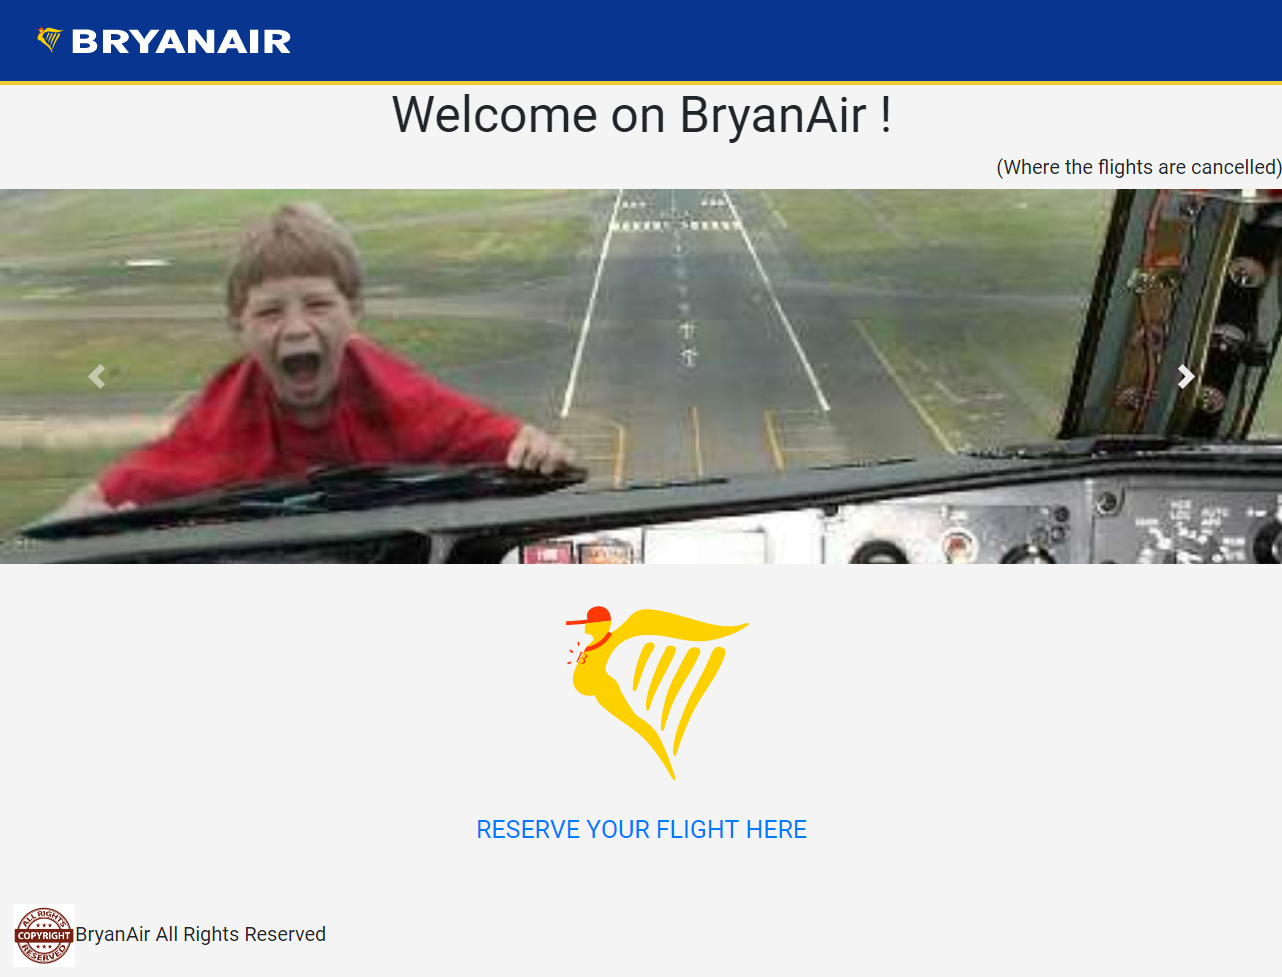
\includegraphics[width=\textwidth]{home.png}
			\caption{Page d'accueil}
			\label{fig:home}
		\end{figure}

		Sur la première page de réservation (figure~\ref{fig:res1}), on peut réserver des billets pour un vol pour plusieurs passagers. Il faut donner l'aéroport de départ et d'arrivée, si on veut un aller simple ou un aller retour, le nombre de passager(s), une adresse email et si on désire une assurance annulation ou pas.
		\begin{figure}
      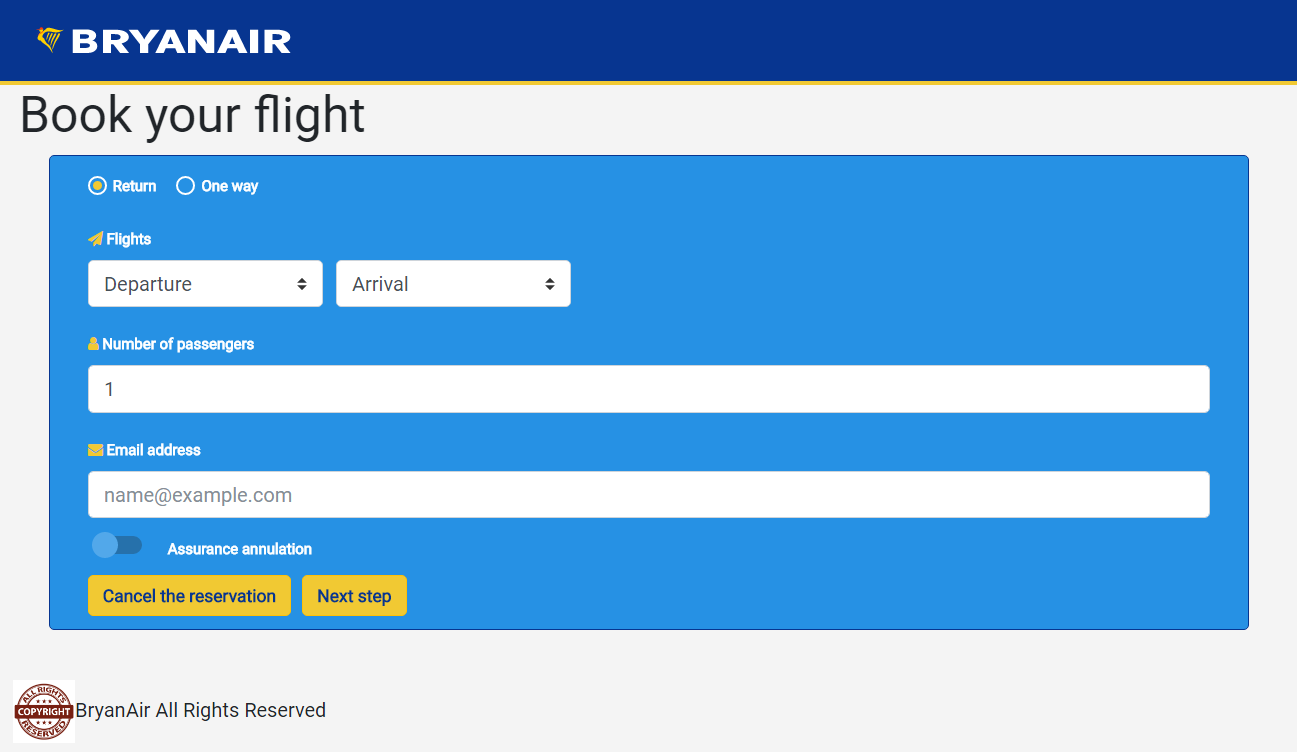
\includegraphics[width=\textwidth]{Reservation.png}
			\caption{Réservation étape 1}
			\label{fig:res1}
		\end{figure}

		La deuxième étape de réservation (figure~\ref{fig:res2}) consiste à enregistrer les informations pour chaque passager tel que le nom, le prénom et l'age.
		\begin{figure}
      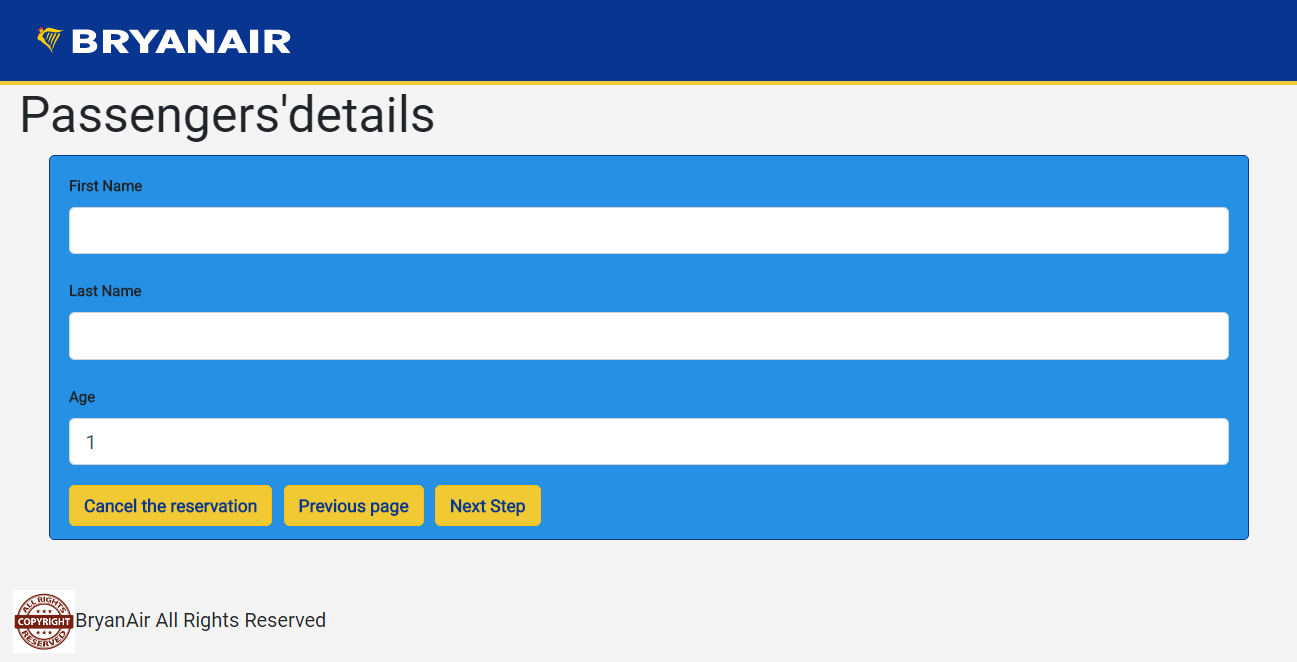
\includegraphics[width=\textwidth]{Detail.png}
			\caption{Réservation étape 2}
			\label{fig:res2}
		\end{figure}

		Une fois tous les passagers enregistrés, on arrive sur une page de confirmation (figure~\ref{fig:conf}) où vous avez le choix de confirmer ou d'annuler votre réservation.

		\begin{figure}
      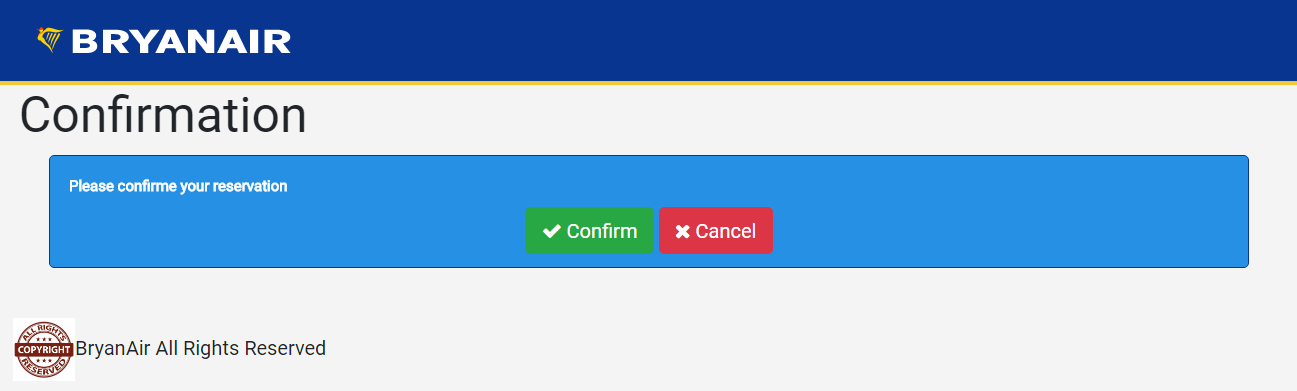
\includegraphics[width=\textwidth]{Confirmation.png}
			\caption{Confirmation}
			\label{fig:conf}
		\end{figure}
		Une fois la réservation confirmée, on arrive sur une page récapitulant la commande (figure~\ref{fig:recap}) avec le prix à payer.
		\begin{figure}
      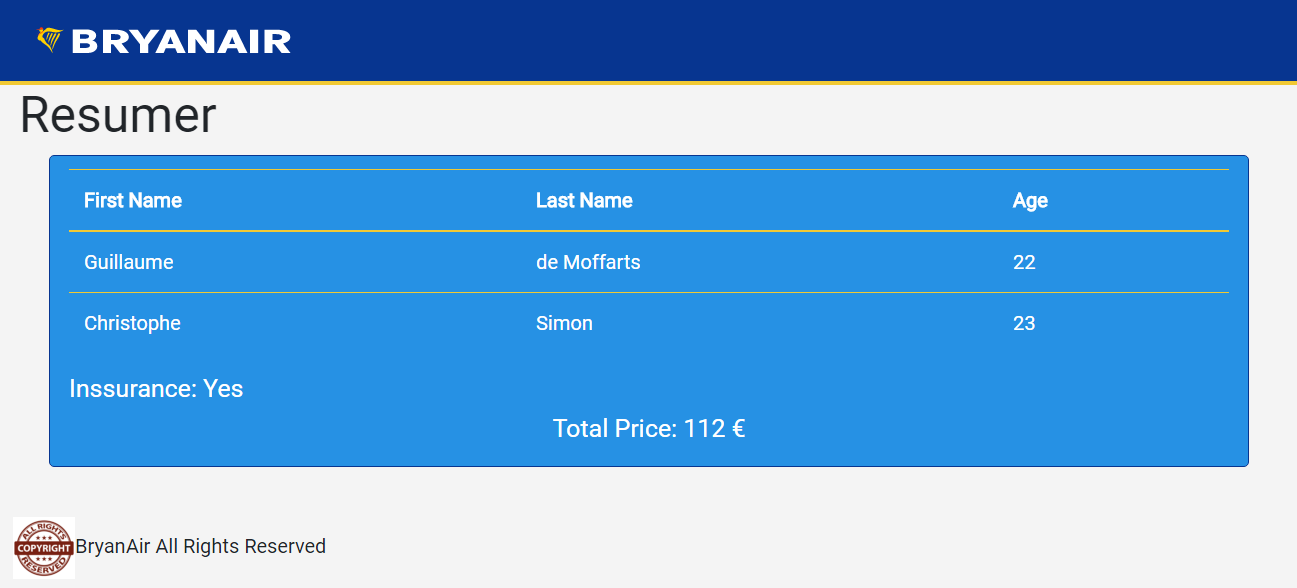
\includegraphics[width=\textwidth]{Resumer.png}
			\caption{Récapitulatif}
			\label{fig:recap}
		\end{figure}

		Enfin, il y a une page d'administration (figure~\ref{fig:admin}) où l'on peut voir, éditer ou supprimer les passagers pour chaque vol. Cette page ne devant pas être accessible au public, il n'y a pas de bouton pour y accéder. On y accède donc uniquement via \url{http://localhost/BryanAir/admin}.

		\begin{figure}
      \includegraphics[width=\textwidth]{admin.png}
			\caption{Page admin}
			\label{fig:admin}
		\end{figure}

	\section{Fonctionnement}
		Dans cette section, vous retrouvez les explications sur le fonctionnement des différentes parties de l'application, tels que la redirection d'URL, les réservations, la page d'administration et les templates html.
		\subsection*{Redirection}
		La conception de l'application est basé sur le design pattern MVC. Nous avons donc un routeur, des modèles, des contrôleurs et des vues. Le routeur redirige vers le contrôleur adéquat grace a a la variable HTTP \texttt{GET}. Il va vérifier les informations venant des formulaires, charger et enregistrer les informations dans la base de données, et va ensuite afficher la page demandée.

		Lorsque qu'on veux accéder à une page, il suffit d'utiliser l'URL suivante \url{localhost/BryanAir/<nom_de_page>}. Cette URL est redirigée vers \url{localhost/Bryanair?page=<nom_de_page>} pour que le routeur puisse rediriger vers le bon contrôleur. Nous avons fait ce choix pour qu'il soit plus facile d'accéder aux différentes pages de l'application. Cette redirection se fait grace a du regex et est configurée dans le fichier \texttt{.htacces}.

		\subsection*{Templates}
		Pour faciliter la construction des vues, nous avons utilisé un sytème de templates html. Nous avons placé des balises comme suit \texttt{\$balise\$} dans nos pages html. Celles-ci vont être remplacées par le contrôleur. La fonction \texttt{buildHTML} dans le fichier \texttt{utils.php}(annexe~\ref{ann:other}) construit d'abord la page en concaténant quatres fichiers HTML. Trois de ces fichiers sont communs pour toutes les pages, il y a le \texttt{head.html}, le \texttt{header.html} et le \texttt{footer.html} (annexe~\ref{ann:tmp}).  Entre ces deux derniers, la vue propre de chaque page est ajoutée.
		On remplace ensuite toutes les balises, grâce aux expressions régulières (regex), par des bouts d'HTML construits par le contrôleur de chaque page. Cette fonction prend en paramètre un liste de clefs/valeurs, les clefs correspondent aux mots dans les balises dans l'HTML et les valeurs contiennent donc le contenu à remplacer.

		Cette méthode permet de faciliter grandement la création des vues. En effet, il ne sera pas nécésaire de copier dans tous les fichiers html un bout de code commun à toutes les pages. Cette méthode permet aussi de bien séparer la partie statique des vue de la partie dynamique gérer par le contrôleur.

		\subsection{Réservation}
      Lorsque vous effectuez une reservation en cliquant sur le bouton réservation de la page d'acceuil, le contrôleur (controle\_reservation.php) charge la liste de tous les aéroports présents dans la table \texttt{airport} de base de donées. Le contrôleur va ensuite construire, comme expliquer ci dessus, la page de réservation grâce à cette liste.

			Lorsque l'utilisateur valide la première page de réservation (figure~\ref{fig:res1}), un contrôleur (controleur\_detail.php) vérifie tout d'abord les données venant du \texttt{POST}. En effet si on passe bien par le formulaire, il ne devrait pas avoir de problème mais on peut tout à fait utiliser un outil tel que curl pour envoyer n'importe quelle requète POST au serveur ou tout simplement changer l'html dans l'inspecteur du navigateur pour pouvoir envoyer du text au lieu d'un entier par exemple. Il faut donc bien vérifier que toutes les données de la requète \texttt{POST} nécessaires au contrôleur ont bien été définies et que le type de chacune est correct. Par exemple, la variable contenant le nombre de passagers doit pouvoir ètre convertie en un entier. Si un problème survient dans la vérification des données, vous êtes redirigés vers la page précédente avec un message d'erreur sur le haut de celle-ci (figure~\ref{fig:error}. Si la vérification est réussie, le contrôleur cherche dans la base de données les numéros de vols (aller/retour) et le nombre de places restantes. S'il n'y a plus de place pour le vol aller ou retour, ou qu'il ne trouve pas de vol pour les aéroports sélectionnés,  un message d'erreur apparaitra comme décrit précédement. Toutes ces informations sont utilisées pour instancier un objet de type \texttt{Reservation} ainsi que deux object \texttt{Flight} et en définir leurs état. Le contrôleur va ensuite construire la page HTML (detail.html) grâce à la fonction expliquée dans la section précédente.

      Vous pouvez retrouver les contrôleurs en annexe~\ref{ann:ctr}
			\begin{figure}
         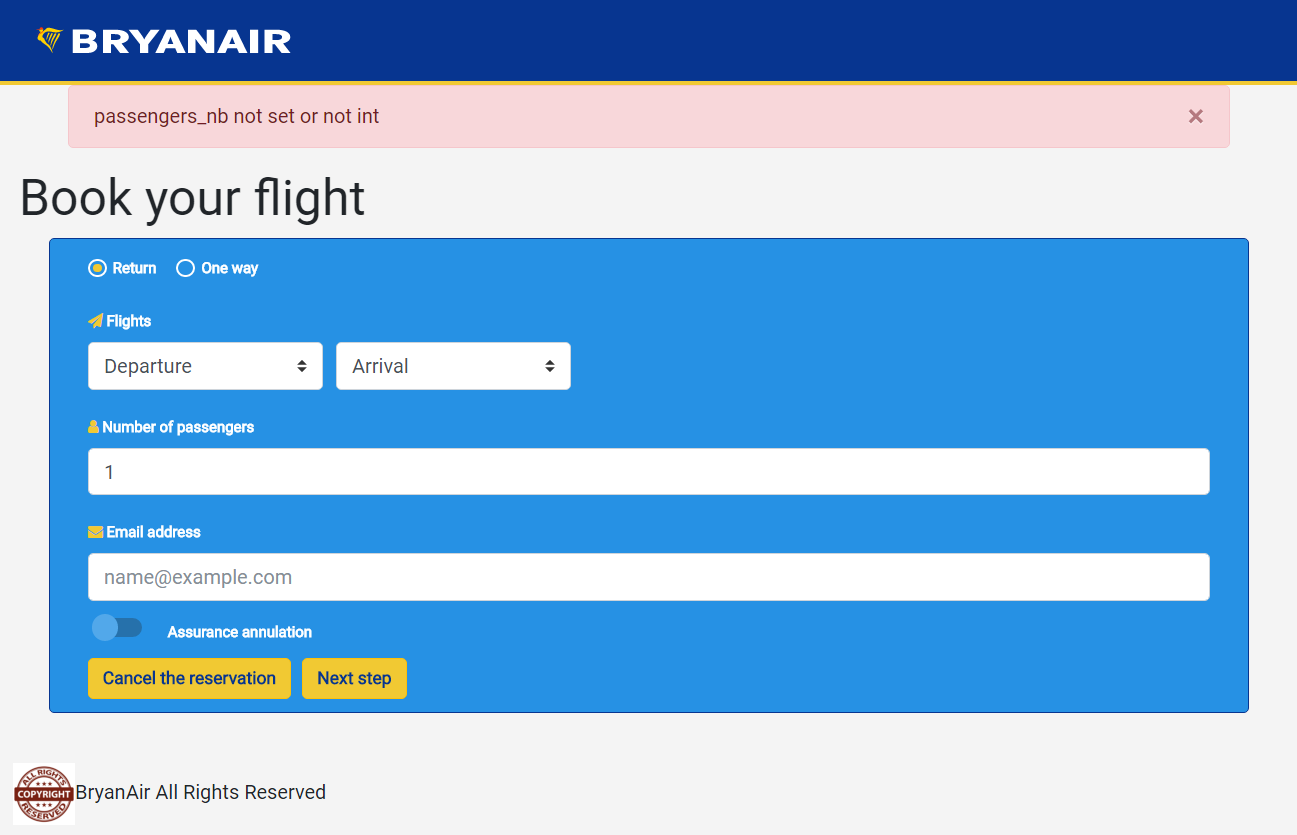
\includegraphics[width=\textwidth]{Error.png}
				\caption{Message d'erreur}
				\label{fig:error}
			\end{figure}

			Nous sommes maintenant arrivés à la deuxième étape de la réservation (figure~\ref{fig:res2}) où il faut encoder une à une les informations sur les passagers. Comme pour la première étape, un contrôleur (controleur\_nextpassenger.php) vérifie les informations de la variable \texttt{HTTP POST}, le même système d'erreur que précédament est d'application. Une fois la vérification passée, le contrôleur instancie un objet de type \texttt{Client} dont l'état est défini par les informations entrées dans le formulaire. Cet objet client est ensuite ajouter dans la liste de clients de l'objet réservation. S'il y a encore des passagers à enregistrer, le contrôleur contruit la même page html que précédemment pour enregistrer un nouveau passager. Si tous les passagers sont enregistrés, le contrôleur construit la page de confirmation (confirmation.html).

			Une fois arrivé sur la page de confirmation (figure~\ref{fig:conf}), on a le choix entre confirmer la réservation ou l'annuler. Si la réservation est annulée, on est redirigé vers la page d'accueil et l'objet réservation avec la liste des clients est supprimé. Si on confirme la réservation, un contrôleur (controleur\_confirmation.php) vérifie si au moins un des passagers est bien majeur. Si ce n'est pas le cas, le système d'erreur affiche un message (figure~\ref{fig:ageError}), il faudra ré-encoder les informations de tous passagers. S'il y a bien au moins une personne majeur, le contrôleur enregistre les clients ainsi que leur réservation (une réservation par client) dans la base de données et va ensuite nous rediriger vers une page résumant la réservation(figure~\ref{fig:recap}).

			\begin{figure}
        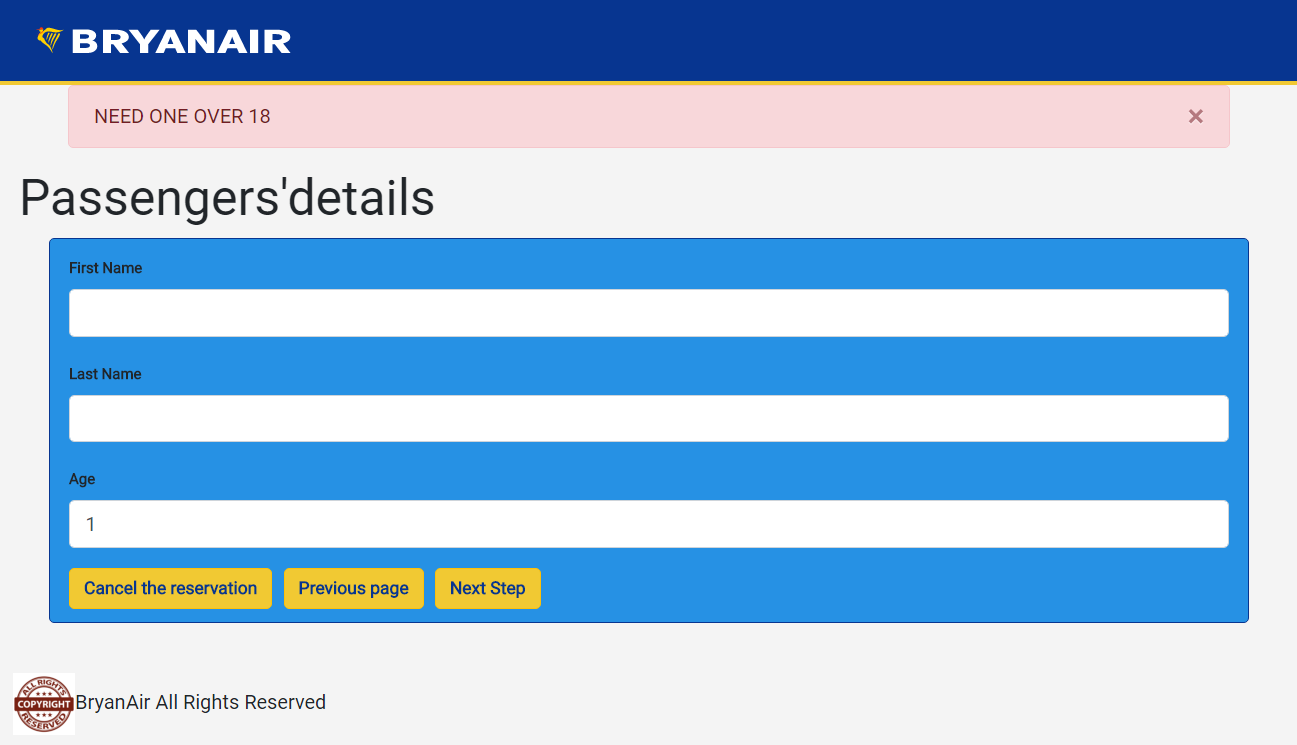
\includegraphics[width=\textwidth]{ageError.png}
				\caption{Erreur de majorité}
				\label{fig:ageError}
			\end{figure}

			Le contrôleur (controleur\_resumer.php) permettant d'afficher cette page va tout d'abord construire un tableau html, avec tous les client contenu dans la réservation, grâce à l'objet réservation. Cet objet se charge aussi de calculer le prix total à payer en se basant sur le nombre de passagers, s'ils ont pris un vol aller retour ou aller simple et enfin, si une assurance annulation est prise. Le contrôleur va ensuite construire la page avec toutes ces informations.

		\subsection{Admin}
			En allant sur la page admin, le contrôleur (controler\_admin.php) charge depuis la base de données tous les vols ainsi que les passagers pour chacun d'entre eux. Il en fait un tableau html représantant toutes ces données puis construit la page html (admin.html).

	\section*{Conclusion}
			Nous pensons avoir respecté toutes les consignes dans le développement de cette application web (au moins toutes les pages demandées, la gestion des erreurs, une feuille de style externe, ...).

			Nous avons fait quelques efforts concernant le style de l'application en utilisant Bootstrap pour les différents boutons, les formulaires, les tableaux, ... Quelques efforts ont également été apportés pour s'approcher le plus possible du site de Ryanair comme le logo et l'icône tous les deux réaliser sous format vectoriel.

      Nous avons intégré une page error 404 pour les erreurs éponymes c'est à dire si l'on cherche une page qui n'existe pas sur BryanAir. Il y a également la possibilité de retourner à la page d'accueil depuis n'importe quelle page en cliquant sur le le logo présents dans le coin supérieur gauche de toutes les pages.

			Cependant, nous pouvons penser à de possibles améliorations pour rendre l'application plus agréable à utiliser. Premièrement, ne pas devoir réencoder toutes les données des passagers quand on revient sur la page réservation depuis la page details ou si au moins un des passagers n'est pas majeur. Ensuite, nous pourrions penser à permettre la modification de la prise de l'assurance annulation depuis la page admin. Cette fonctionnalité n'est pas possible pour le moment à cause de la structure de la base de données. Pour terminer, nous aurions pu mettre le résumer de la réservation sur la page de confirmation pour confirmer avec sa réservation sous les yeux.

			Ce travail nous a apporté une meilleur connaissance du développement web et plus particulièrement du modéle de développement MVC. Nous avons également pu nous familiariser avec de la création et la manipulation d'une base de données Mysql.
\pagebreak
  \appendix
  \section{Modèles \label{ann:mdl}}
    \subsection{Client.php}
    \lstinputlisting[language=php]{\file{models/Client.php}}
    \subsection{Flight.php}
    \lstinputlisting[language=php]{\file{models/Flight.php}}
    \subsection{Reservation.php}
    \lstinputlisting[language=php]{\file{models/Reservation.php}}
\section{templates \label{ann:tmp}}
  \subsection{home.html}
  \lstinputlisting[language=html]{\file{templates/home.html}}
  \subsection{reservation.html}
  \lstinputlisting[language=html]{\file{templates/reservation.html}}
  \subsection{detail.html}
  \lstinputlisting[language=html]{\file{templates/detail.html}}
  \subsection{confirmation.html}
  \lstinputlisting[language=html]{\file{templates/confirmation.html}}
  \subsection{resumer.html}
  \lstinputlisting[language=html]{\file{templates/resumer.html}}
  \subsection{admin.html}
  \lstinputlisting[language=html]{\file{templates/admin.html}}
  \subsection{head.html}
  \lstinputlisting[language=html]{\file{templates/head.html}}
  \subsection{header.html}
  \lstinputlisting[language=html]{\file{templates/header.html}}
  \subsection{footer.html}
  \lstinputlisting[language=html]{\file{templates/footer.html}}
  \subsection{admin.html}
  \lstinputlisting[language=html]{\file{templates/admin.html}}

\section{Controlers \label{ann:ctr}}
  \subsection{controler\_home.php}
  \lstinputlisting[language=php]{\file{controler_home.php}}
  \subsection{controle\_reservation.php}
  \lstinputlisting[language=php]{\file{controler_reservation.php}}
  \subsection{controler\_detail.php}
  \lstinputlisting[language=php]{\file{controler_detail.php}}
  \subsection{controler\_nextpassenger.php}
  \lstinputlisting[language=php]{\file{controler_nextpassenger.php}}
  \subsection{controler\_confirmation.php}
  \lstinputlisting[language=php]{\file{controler_confirmation.php}}
  \subsection{controler\_resumer.php}
  \lstinputlisting[language=php]{\file{controler_resumer.php}}
  \subsection{controler\_admin.php}
  \lstinputlisting[language=php]{\file{controler_admin.php}}
  \subsection{controler\_update.php}
  \lstinputlisting[language=php]{\file{controler_update.php}}
  \subsection{controler\_delete.php}
  \lstinputlisting[language=php]{\file{controler_delete.php}}
  \subsection{controler\_404.php}
  \lstinputlisting[language=php]{\file{controler_404.php}}

\section{Other \label{ann:other}}
  \subsection{.htaccess}
  \lstinputlisting[language={}]{\file{.htaccess}}
  \subsection{index.php}
  \lstinputlisting[language=php]{\file{index.php}}
  \subsection{utils.php}
  \lstinputlisting[language=php]{\file{utils.php}}
  \subsection{style.css}
  \lstinputlisting[language=css]{\file{ressources/CSS/style.css}}
\end{document}
